\documentclass[
	german,%globale Übergabe der Hauptsprache
%	logofile=example-image-duck, %Falls die Logo Dateien nicht vorliegen
	authorontitle=true,
	]{bfhbeamer}


\usepackage[main=german]{babel}
\usepackage{caption}

% Der folgende Block ist nur bei pdfTeX auf Versionen vor April 2018 notwendig
\usepackage{iftex}
\ifPDFTeX
\usepackage[utf8]{inputenc}%kompatibilität mit TeX Versionen vor April 2018
\fi


%Makros für Formatierungen der Doku
%Im Allgemeinen nicht notwendig!
\let\code\texttt

\title{Bachelor Thesis}
\subtitle{Unlinkability of Verifiable Credentials in a practical approach}
\author[J. Robles]{Joel Robles - Adv. Dr. Annett Laube, Dr. Reto Koenig - Exp. Dr. Andreas Spichiger | TI}
% \institute{TI}
\titlegraphic*{\includegraphics{example-image-duck}}%is only used with BFH-graphic and BFH-fullgraphic
\date{3. Juli, 2024}

% \setbeamertemplate{page number in foot}[framenumber]

%Activate the output of a frame number:
\setbeamertemplate{footline}[frame number]


\AtBeginSection{\sectionpage}

\begin{document}

\maketitle

\begin{frame}{Inhaltsverzeichnis}
    \tableofcontents
\end{frame}

\section{Ziel}

\begin{frame}{Was ist das Ziel?}
    \centering
    Die Analyse, ob eine Implementierung von Verifiable Credentials mit dem BBS Signature Scheme in der realen Welt Unverknüpfbarkeit beibehält
\end{frame}

\section{Self-sovereign Identity}

\begin{frame}{Self-sovereign Identity (SSI)}
    \begin{itemize}
        \item Ist ein Konzept, bei dem eine Person (\textbf{Holder}) entscheiden kann, wer was über sie wissen darf
        \item Holder dürfen wählen, was sie offenbaren und was nicht (\textbf{selective disclosure})
        \item Keine Verbindung zwischen Präsentationen (\textbf{unlinkability})
        \item Heutiger Stand - Holder haben keine Kontrolle über ihre Attribute
        \item Zukünftiger Stand dank SSI - Holder haben volle Kontrolle über ihre Attribute
    \end{itemize}
\end{frame}

\begin{frame}{Trust Triangle}
    \begin{columns}[onlytextwidth,T]
        \column{70mm}  
        \begin{itemize}
            \item Der Holder zeigt einem Verifier eine staatliche ID 
            \item Diese beinhaltet mehrere Attribute, z.B. Vorname
            \item Wie weiss ein Verifier, dass eine Menge von Attributen (\textbf{Credential}) valid ist?
            \item Er vertraut dem Issuer!
            \item Beispiel: Schweizer ID hat Hologramme
        \end{itemize}

        \column{70mm}

        \begin{figure}
            \centering
            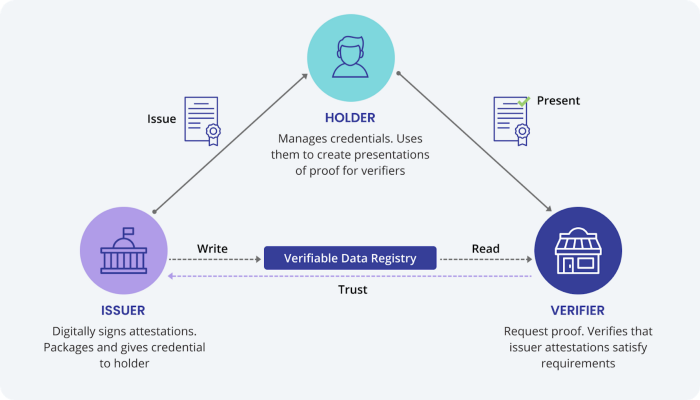
\includegraphics[width=70mm]{../img/trusttriangle.png}
            \caption{Trust triangle}
        \end{figure}
        
    \end{columns}
\end{frame}

\section{Verifiable Credentials \& Verifiable Presentations}

\begin{frame}{Verifiable Credentials (VC)}
    \begin{columns}[onlytextwidth,T]
        \column{70mm}  

    \begin{itemize}
        \item Verifiable Credentials sind eine digitale Repräsentation von physischen Credentials
    \end{itemize}

    \column{70mm}
    \begin{figure}
        \centering
        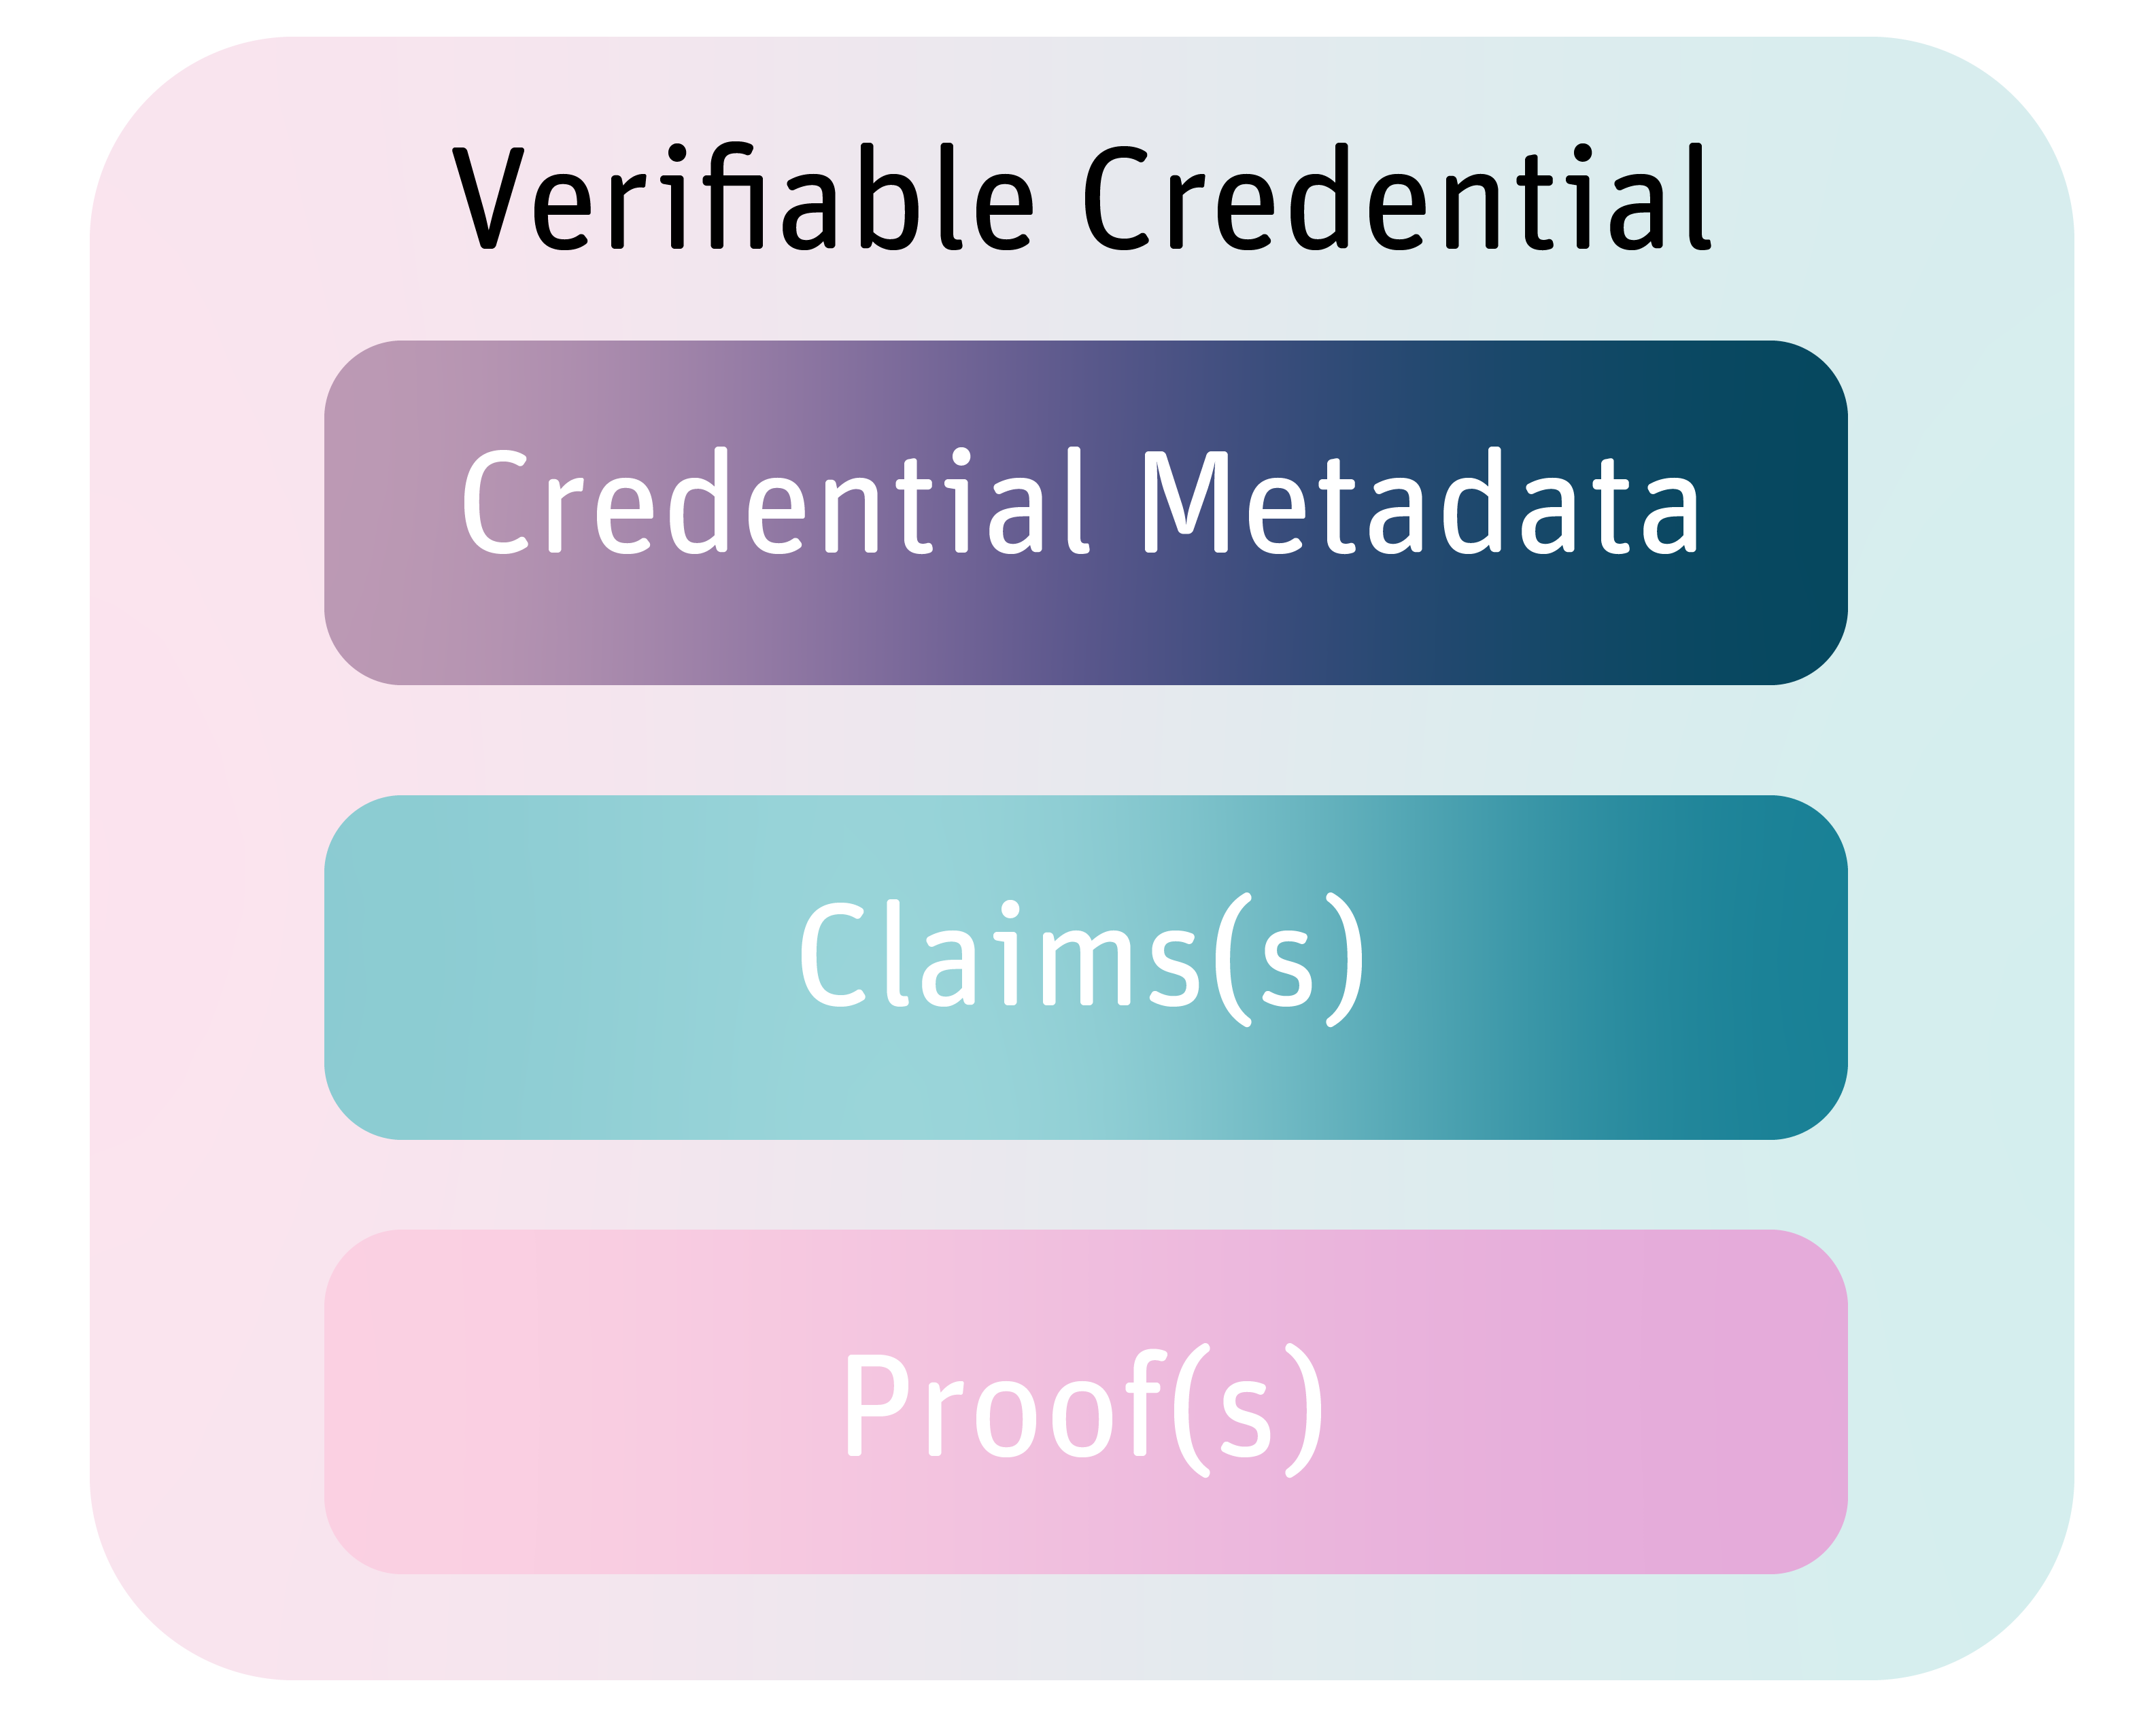
\includegraphics[width=70mm]{../img/VC.png}
        \caption{VC Aufbau}
    \end{figure}

    \end{columns}
\end{frame}

\begin{frame}{Verifiable Credentials (VC)}
    \begin{columns}[onlytextwidth,T]
        \column{70mm}  

    \begin{itemize}
        \item Verifiable Credentials sind eine digitale Repräsentation von physischen Credentials
        \item JSON-LD repräsentiert Attribute als \textbf{key-value pairs}
        \item Beispiel:
        \begin{itemize}
            \item Vorname auf einer ID
            \item Repräsentiert als \{"first\_name": "John"\}
            \item ``first\_name'' ist der key und ``John'' ist der value
        \end{itemize}
    \end{itemize}

    \column{70mm}
    \begin{figure}
        \centering
        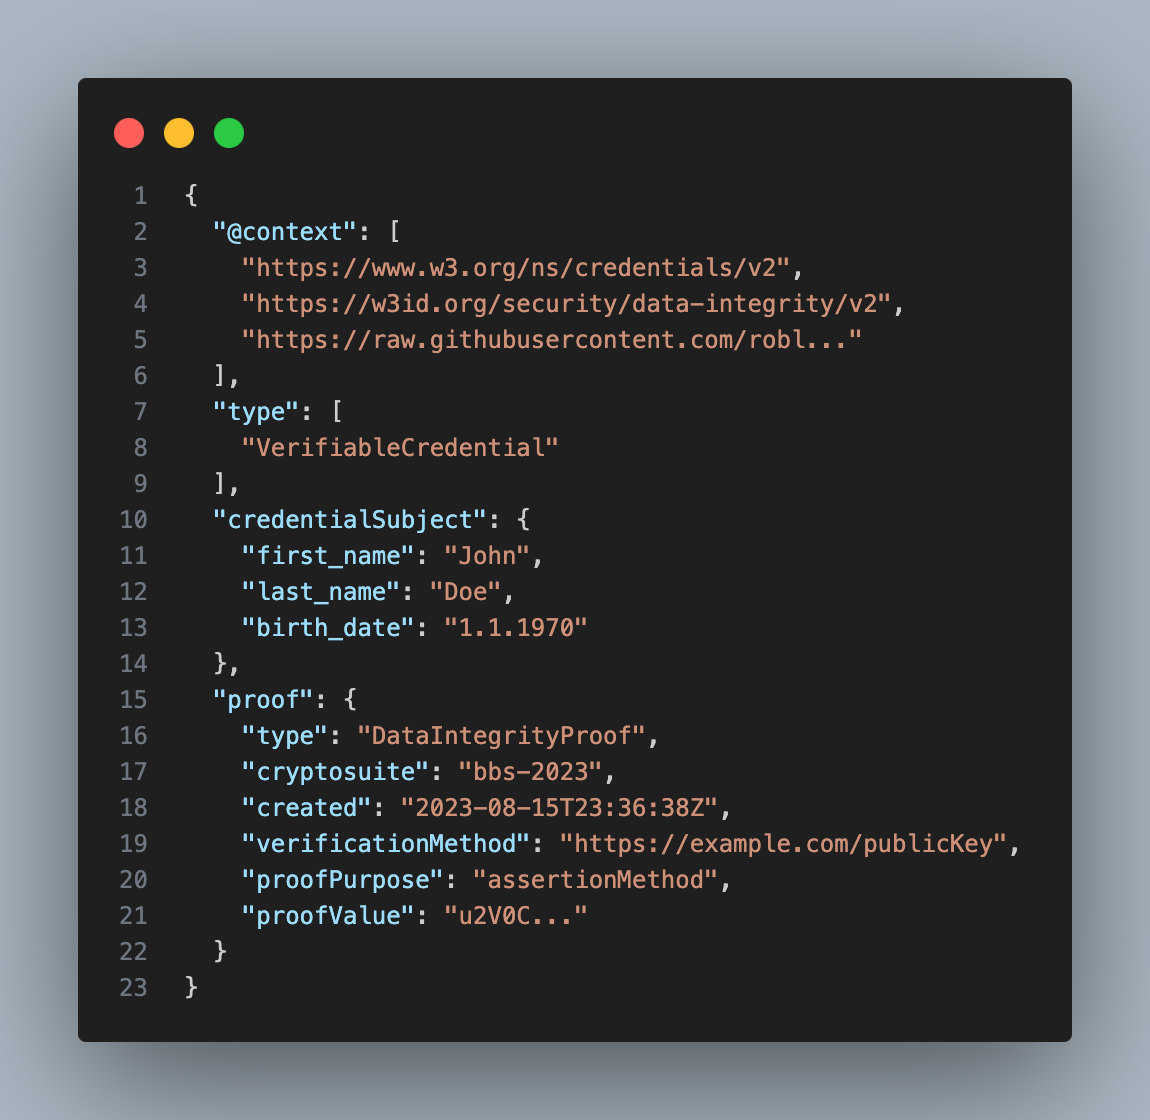
\includegraphics[width=60mm]{../img/VCSignExample.png}
        \caption{Beispiel VC}
    \end{figure}

    \end{columns}
\end{frame}

\begin{frame}{Probleme von digitalen Credentials}
    \begin{columns}[onlytextwidth,T]
        \column{70mm}  
        \textbf{Problem 1:}
        \begin{itemize}
            \item Holder zeigt ein Credential einem Verifier
            \item Der Verifier, sieht alle Attribute
            \item Bricht \textbf{selective-disclosure}
        \end{itemize}

        \column{70mm}  
        \textbf{Problem 2:}
        \begin{itemize}
            \item Holder zeigt ein Credential einem Verifier
            \item Holder zeigt das gleiche Credential einem zweiten Verifier
            \item Der Holder kann ge-linked werden (Metadaten)
            \item Bricht \textbf{unlinkability}
        \end{itemize}

    \end{columns}
\end{frame}


\begin{frame}{VCs and BBS}
    \begin{itemize}
        \item Warum werden sie \textbf{Verifiable} Credentials genannt?
        \item Der Verifier kann ein VC, welches ihm präsentiert wurde (\textbf{Verifiable Presentation}), aufgrund kryptographischer Signaturen verifizieren
        \item Diese zeigen, dass das Credential seit der Ausstellung nicht verändert wurde
        \item Wir nutzen das BBS Signature Scheme (\textbf{BBS}) 
        \item Dieses Schema bietet \textbf{selective disclosure} und \textbf{unlinkability}
        \item Aber wie unlinkability? - Der Verifier braucht die Signatur
        \item BBS kann \textbf{proofs} generieren
        \item Diese beweisen, dass der Holder die Signatur kennt, ohne diese zu offenbaren
        \item Fungieren als neue Signatur für das selectively disclosed VC
        \item Weiter sind proofs unverknüpfbar zwischen jeder Generierung
    \end{itemize}
\end{frame}

\begin{frame}{BBS proofs}
    \centering
    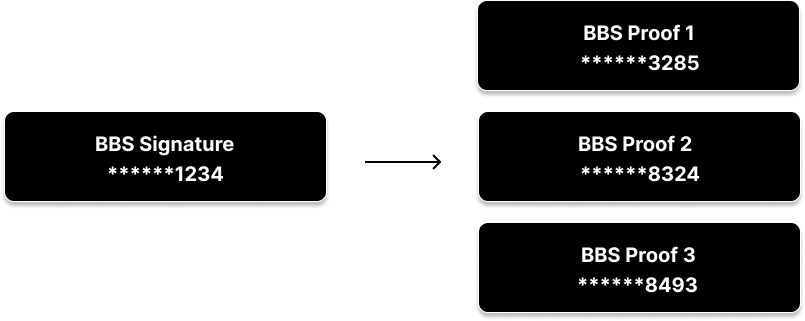
\includegraphics[width=120mm]{../img/BBSProofGen.png}
\end{frame}

\begin{frame}{BBS proofs}
    \begin{columns}[onlytextwidth,T]
        \column{70mm}  
        \begin{figure}
            \centering
            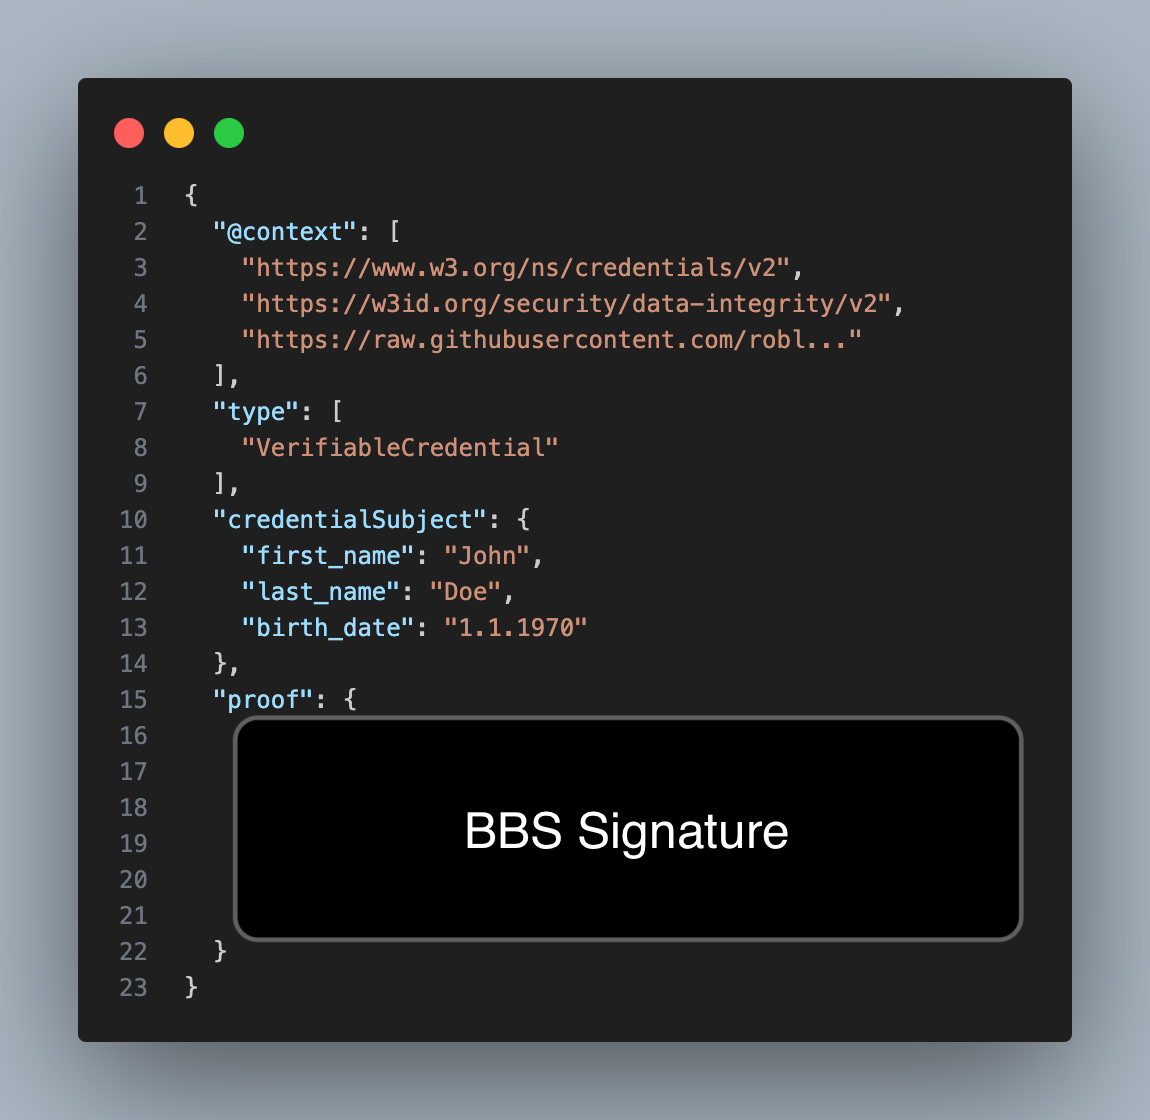
\includegraphics[width=60mm]{../img/VCSignBlock.png}
            \caption{VC mit BBS Signatur}
        \end{figure}

        \column{70mm}

        \begin{figure}
            \centering
            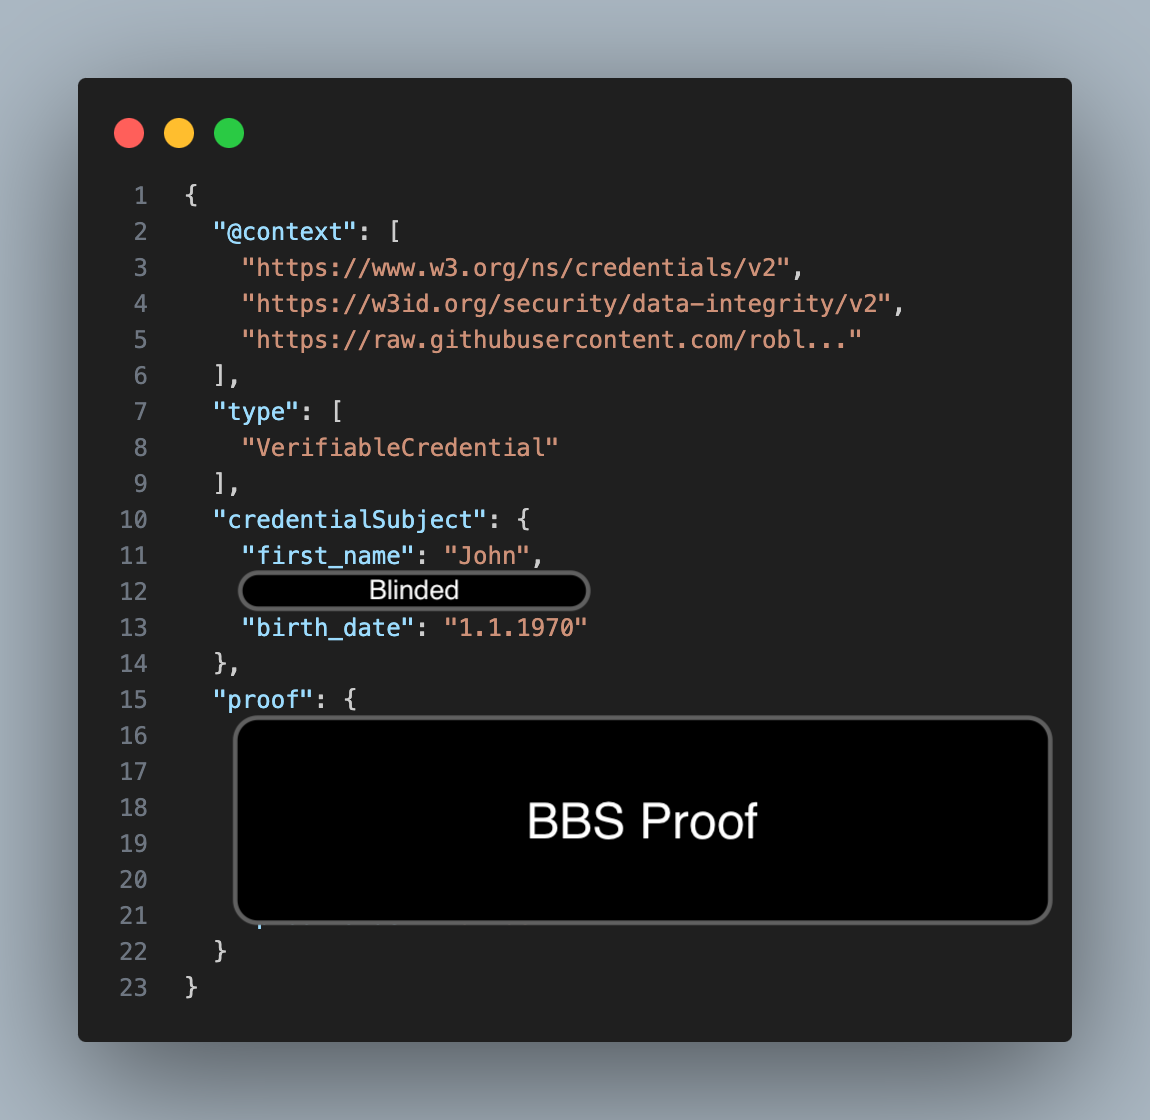
\includegraphics[width=60mm]{../img/VCProofBlock.png}
            \caption{VC mit BBS Proof}
        \end{figure}

    \end{columns}
\end{frame}


\begin{frame}{Verifiable Presentation (VP)}
    \begin{columns}[onlytextwidth,T]
        \column{70mm}  
        \begin{itemize}
            \item Ein Holder würde gerne ein VC präsentieren
            \item Dafür werden \textbf{Verifiable Presentations} genutzt
            \item BBS kann nur Statements signieren
            \item Der \textbf{RDF} canonicalization Algorithmus, welcher Statements aus key-value pairs generiert
        \end{itemize}

        \column{70mm}

        \begin{figure}
            \centering
            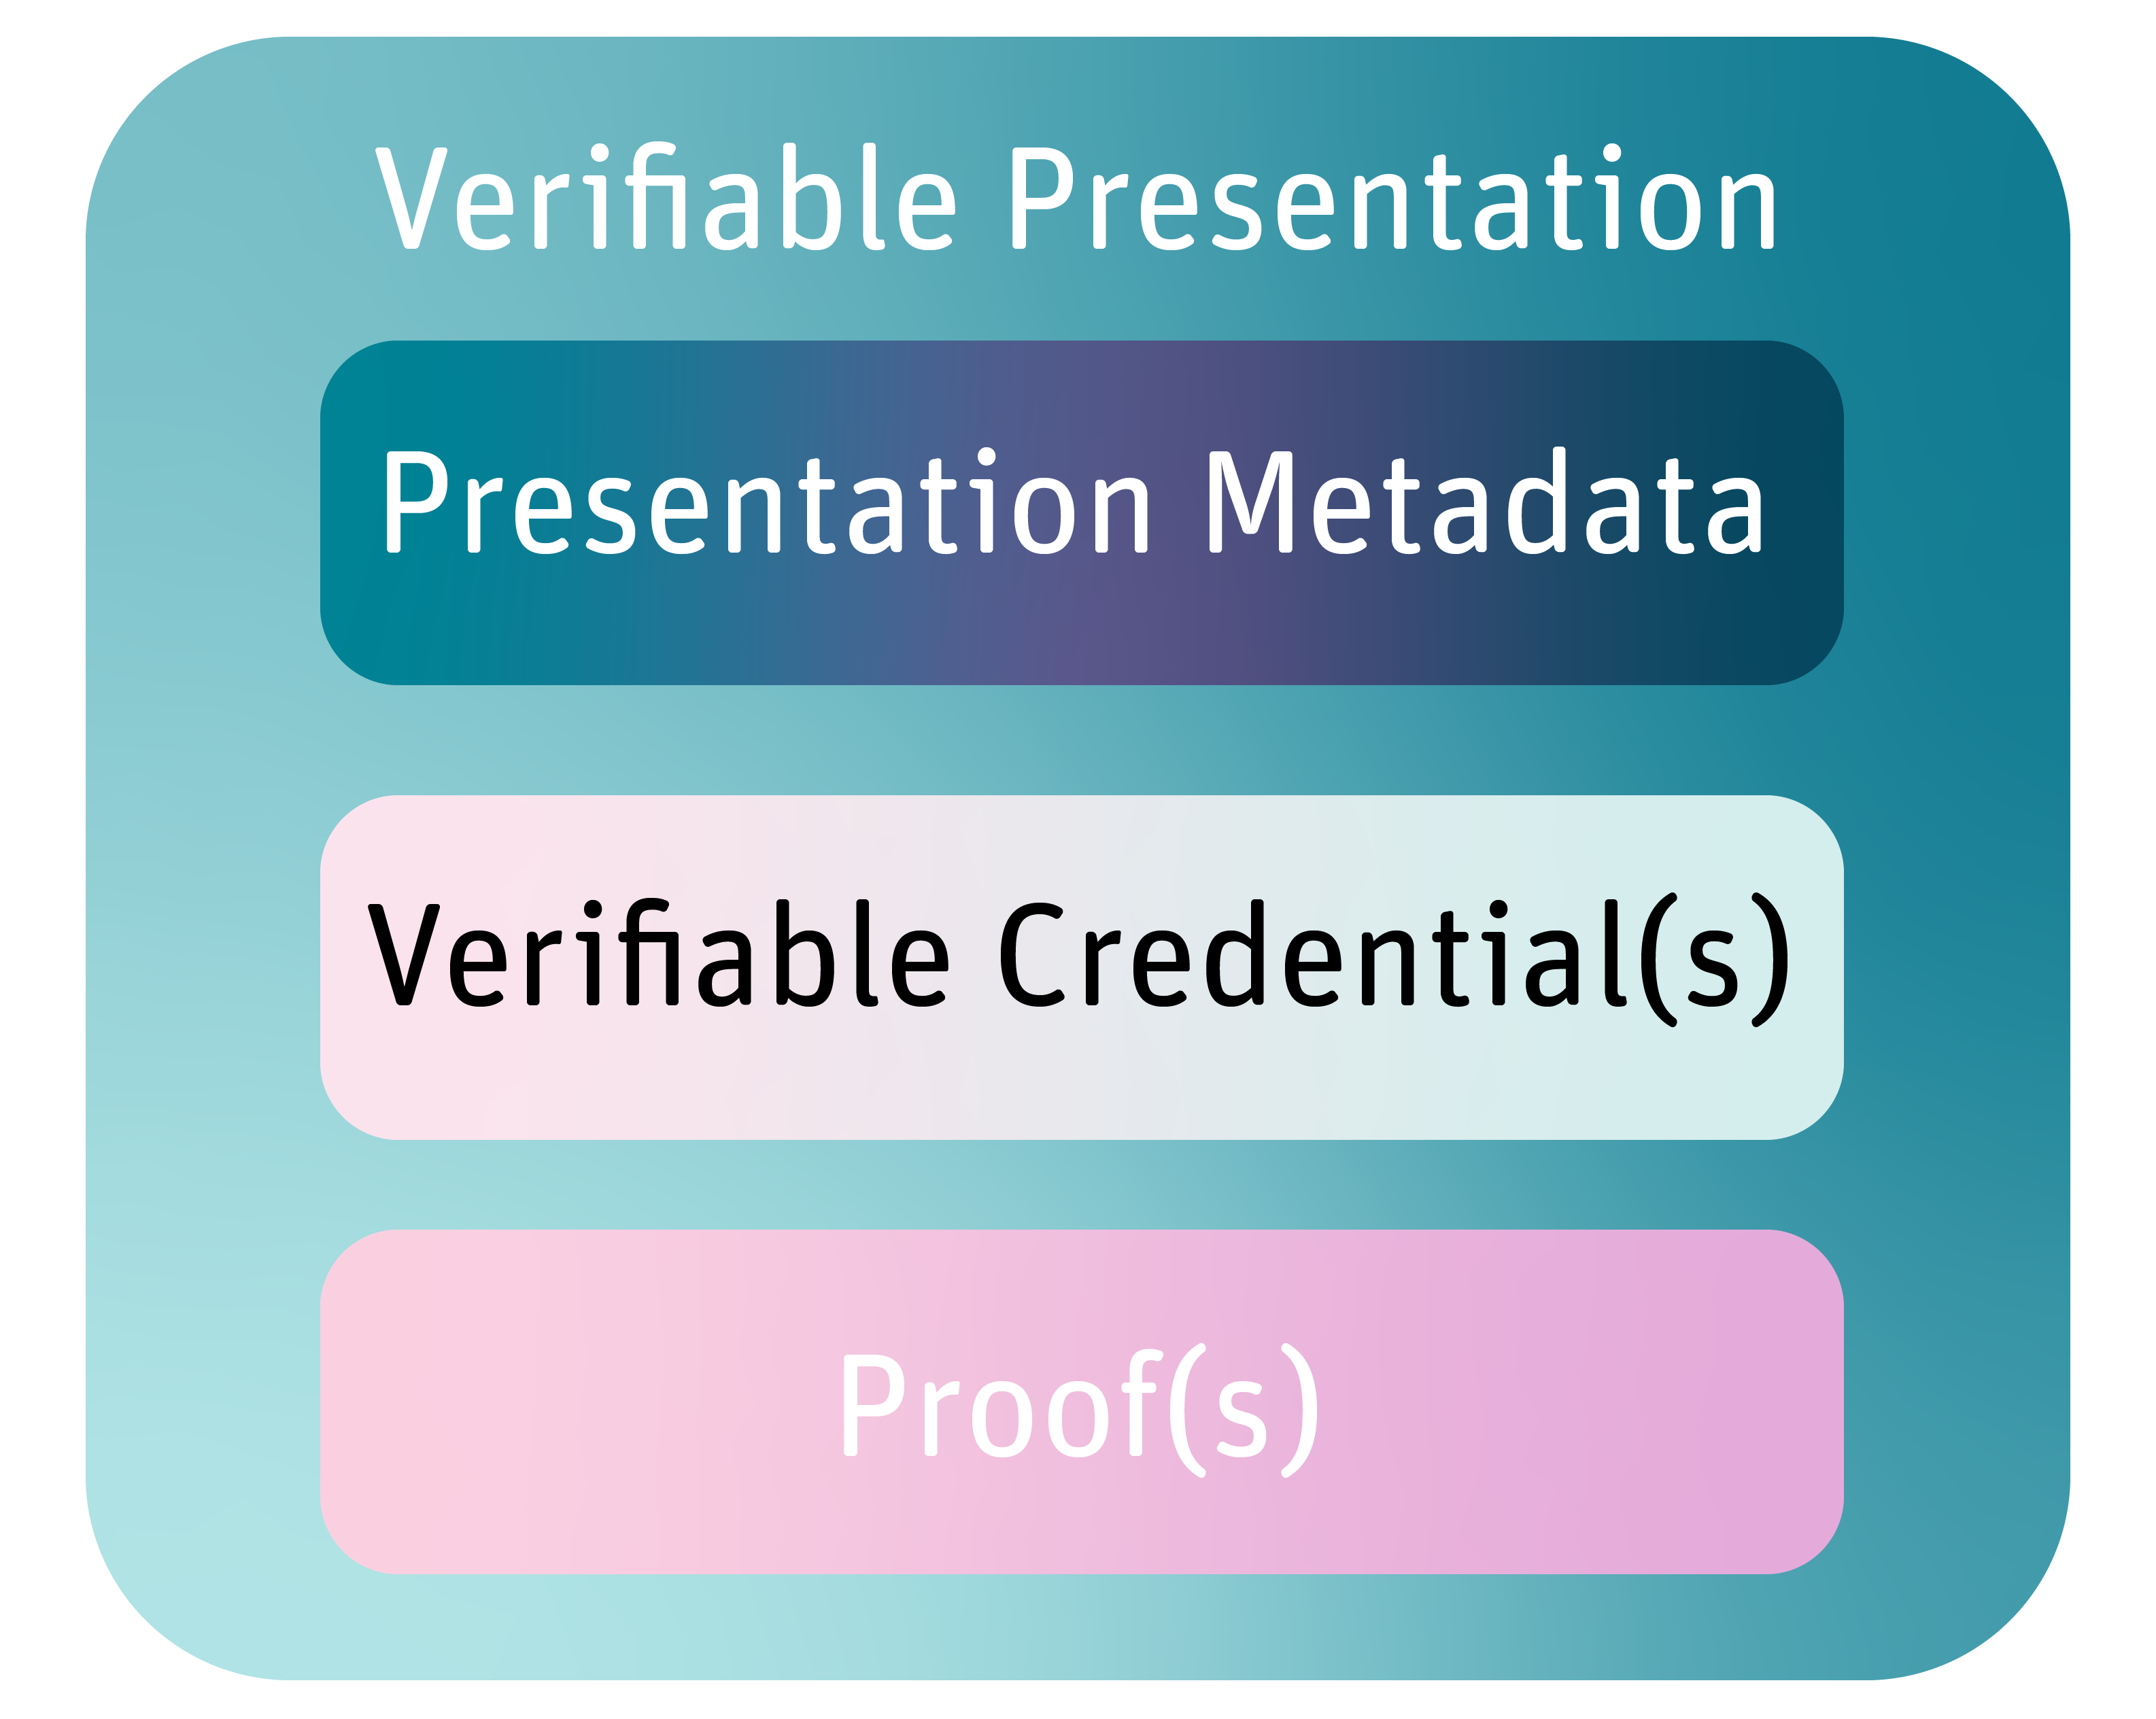
\includegraphics[width=70mm]{../img/VP.png}
            \caption{VP Aufbau}
        \end{figure}

    \end{columns}
\end{frame}

\begin{frame}{Der RDF Algorithmus}
    \centering
    JSON zu Statements
    \begin{columns}[onlytextwidth,T]
        \column{70mm}  
        \begin{figure}
            \centering
            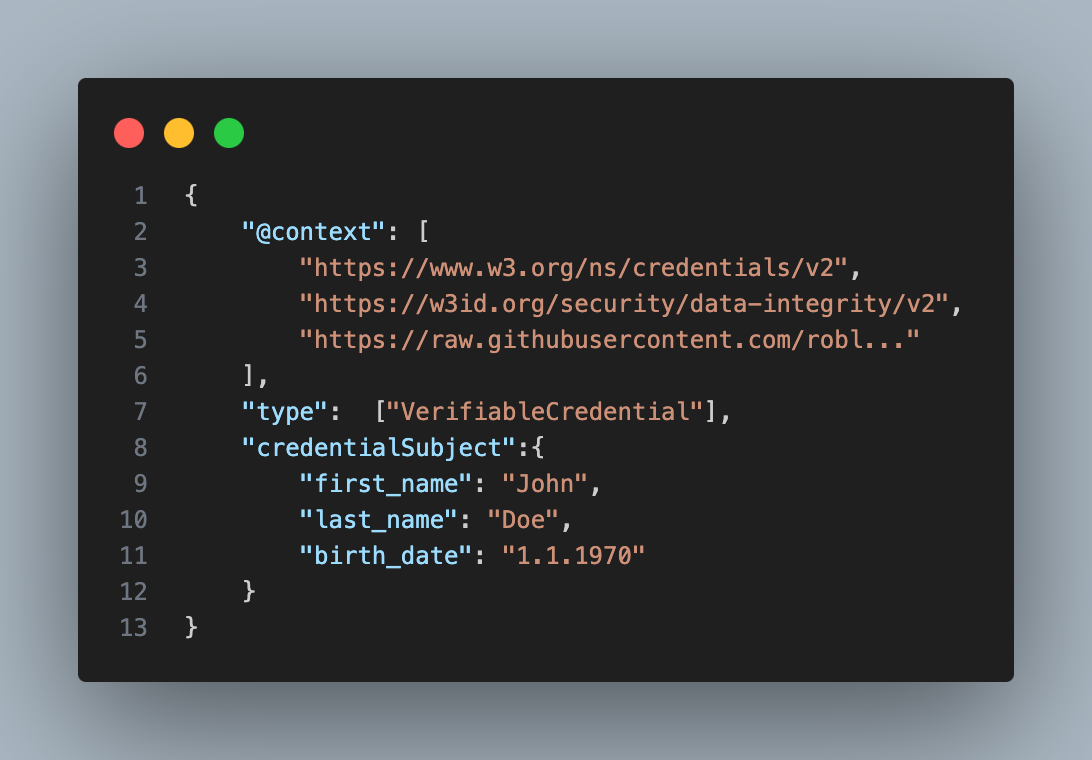
\includegraphics[width=70mm]{../img/VCexp.png}
            \caption{Beispiel VC}
        \end{figure}

        \column{70mm}  
        \begin{figure}
            \centering
            \includegraphics[width=70mm]{../img/Statements.png}
            \caption{Beispiel Statements}
        \end{figure}
    \end{columns}
\end{frame}

\begin{frame}{Der RDF Algorithmus}
    \centering
    Statements sortieren
    \begin{columns}[onlytextwidth,T]
        \column{70mm}  
        \begin{figure}
            \centering
            \includegraphics[width=70mm]{../img/Statements.png}
            \caption{Beispiel Statements}
        \end{figure}

        \column{70mm}  
        \begin{figure}
            \centering
            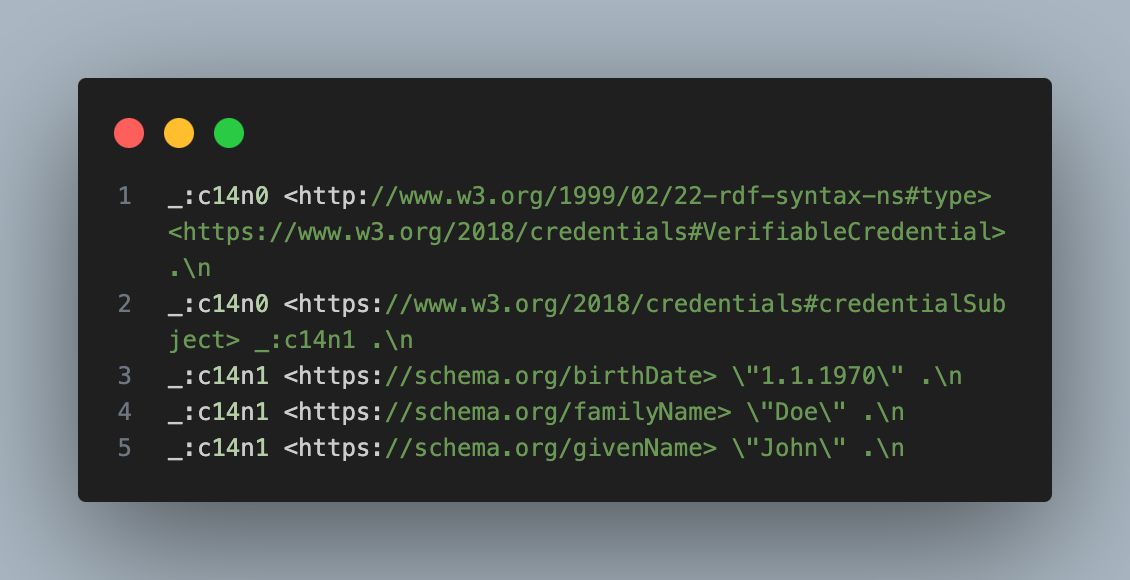
\includegraphics[width=70mm]{../img/hashed.png}
            \caption{Beispiel Sortierung}
        \end{figure}
    \end{columns}
\end{frame}

\begin{frame}{Permutation von Statements}
    \begin{itemize}
        \item Holder bekommt ein VC, welches unter anderem ein Zivilstands-Attribut beinhaltet
        \item Holder präsentiert ein VP mit verborgenen Zivilstands-Attribut
        \item Holder heiratet, bekommt ein neues VC mit geändertem Zivilstand
        \item Holder präsentiert das aktualisierte VP mit verborgenem Zivilstand
        \item \textbf{Datenleck}: Der Verifier kann herausfinden, dass sich der Zivilstand geändert hat
        \item Aber nur wenn Attribute, welche nach dem Zivilstand kommen, präsentiert werden (RDF Algorithmus)
        \item Damit das nicht passieren kann, muss der Issuer immer die Statements zufällig permutieren
        \item Der Issuer muss die Permutation dem Holder bekannt geben, aber \textbf{nie} dem Verifier
    \end{itemize}
\end{frame}

\begin{frame}{Verknüpfbarkeit von Identifikatoren \& Metadaten}
    \begin{itemize}
        \item VCs können Metadaten wie Ablaufdatum beinhalten
        \item Falls das Ablaufdatum sehr genau ist (z.B. auf die Sekunde), führt dies zu Verknüpfbarkeit
        \item Ablaufdatum auf einen Tag genau, um die Verknüpfbarkeit zu umgehen
        \item VCs und VPs können auch IDs für z.B. Entziehung beinhalten, welche zu Verknüpfbarkeit führen
        \item Dafür kan man Zero-Knowledge proofs verwenden, um zu zeigen, dass man nicht Teil einer Entzugs-Liste ist
    \end{itemize}
\end{frame}

\section{OpenID Connect for Verifiable Presentations}

\begin{frame}{Transport zwischen Holder und Verifier}
    \begin{figure}
        \centering
        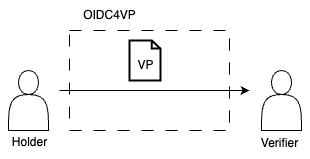
\includegraphics[width=70mm]{../img/OIDC4VP.png}
        \caption{OpenID connect for Verifiable Presentations}
    \end{figure}
\end{frame}

\begin{frame}{OIDC4VP Fluss}
    \begin{figure}
        \centering
        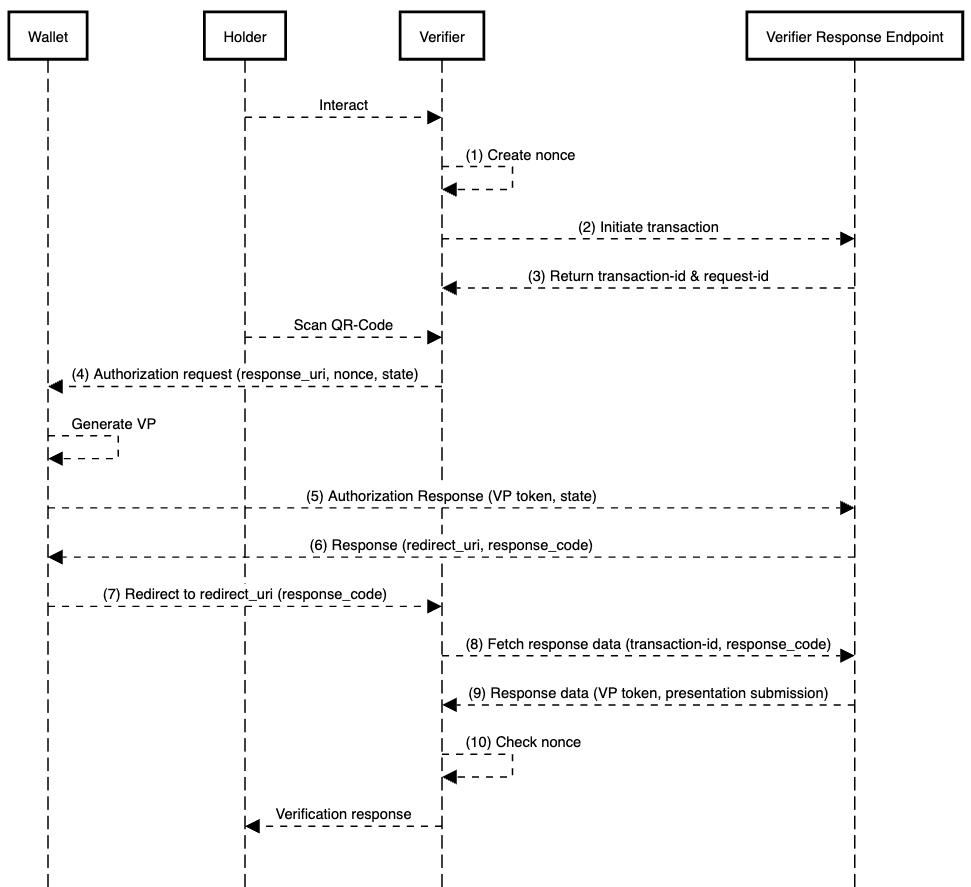
\includegraphics[width=70mm]{../img/OIDC4VPFlow.png}
        \caption{OpenID connect for Verifiable Presentations Sequenz}
    \end{figure}
\end{frame}

\begin{frame}{Replay attack}
    \begin{itemize}
        \item Der Holder sendet dem Verifier ein VP
        \item Ein \textit{Man-in-the-Middle} speichert die Vorstellung
        \item Der \textit{Man-in-the-Middle} kann das gespeicherte VP wiederverwenden
        \item Um dieses Problem zu umgehen, wird eine Zufallszahl genutzt (challenge-response)
    \end{itemize}
\end{frame}

% \begin{frame}{Session fixation attack}
%     \begin{itemize}
%         \item Der Holder legt das VP im Endpoint des Verifiers ab
%         \item Falls das System des Verifiers infisziert ist, kann ein Angreifer das VP einsehen
%         \item Der endpoint des Verifiers retourniert eine redirect URL und ein response code
%         \item Dieser code wird an das Terminal weitergeleitet, somit kann das infiszierte System das VP nicht einsehen
%     \end{itemize}
% \end{frame}

\section{Fazit}

\begin{frame}{Fazit}
    \begin{itemize}
        \item Wie kombiniert man BBS und VCs?
        \begin{itemize}
            \item \textbf{Durch den RDF Algorithmus}
        \end{itemize}
        \item Was sind die Probleme mit dieser Kombination und wie kann man diese lösen?
        \begin{itemize}
            \item \textbf{Determinismus des RDF Algorithmus und Verknüpfbarkeit von Metadaten und Identifikatoren}
            \item \textbf{Lösung: Permutierung der Statements und Gebrauch von zero-knowledge proofs}
        \end{itemize}
        \item Wie werden die VPs von Holder zu Verifier gesendet und was sind die Probleme?
        \begin{itemize}
            \item \textbf{OpenID connect for Verifiable Presentations}
            \item \textbf{Replay-Attacke, gelöst mit der nonce}
        \end{itemize}
    \end{itemize}
\end{frame}

\begin{frame}{Fazit}
    \centering
    \textbf{\huge Es funktioniert!}
\end{frame}

\section{Ausblick}

\begin{frame}{Ausblick}
    \begin{itemize}
        \item Link Secrets und Blind BBS Signatures für linkability und selective disclosure analysieren
        \item Implementieren und testen
    \end{itemize}
\end{frame}

\end{document}